\par
Les QR Codes devant stocker plus d'informations que dans la version initiale de l'application mobile, il nous a fallu définir une structure de données pour les représenter. Cette représentation s'est construite parallèlement à l'élaboration des types de QR Codes (voir \ref{typesQR}) et à celle du Modèle (voir \ref{architecture}), afin d'assurer la cohérence de l'ensemble.\\

\par
Dans le but de minimiser la quantité d'informations contenue dans le QR Code, nous nous sommes appuyés sur un modèle séparant les données nécessaires à la lecture par l'application mobile et les données nécessaires seulement au chargement à l'identique du QR Code après son enregistrement par l'application de bureau.\\

\par
Pour comprendre, prenons l'exemple d'une page d'un livre pour enfant décrivant des animaux. Afin de rendre cette page plus ludique pour les non-voyants, les transcripteurs de l'institut souhaiteraient coller sur cette page un QR Code pour chaque animal décrit. Ces QR Codes contiendraient chacun un petit texte explicatif et le cri de l'animal. Ils souhaiteraient qu'ils soient lus dans un ordre prédéfini, et qu'un texte en braille représentant les lettres \textit{QR} soit présent au centre de chacun des QR Codes. De plus, le QR Code devrait être bleu et le texte central en braille rouge afin qu'il puisse être imprimé en relief.

\par
Parmi ces données, certaines ne sont pas indispensables à l'application mobile pour interpréter le QR Code. Elle n'a par exemple pas besoin de connaître le texte en braille ou le nom du fichier contenant le cri de l'animal. Ces données seront en revanche nécessaires à l'application de bureau pour recharger les QR Codes à l'identique le jour où les transcripteurs voudront modifier la description de l'animal. Nous allons donc séparer ces données en deux parties : les données nécessaires à l'application mobile seront encodées dans le QR Code tandis que les données qui ne le sont pas seront insérées dans le fichier image, mais pas dans le QR Code en lui-même. Nous détaillons cette séparation dans le schéma suivant.



\begin{figure}[!h]
	\centering
   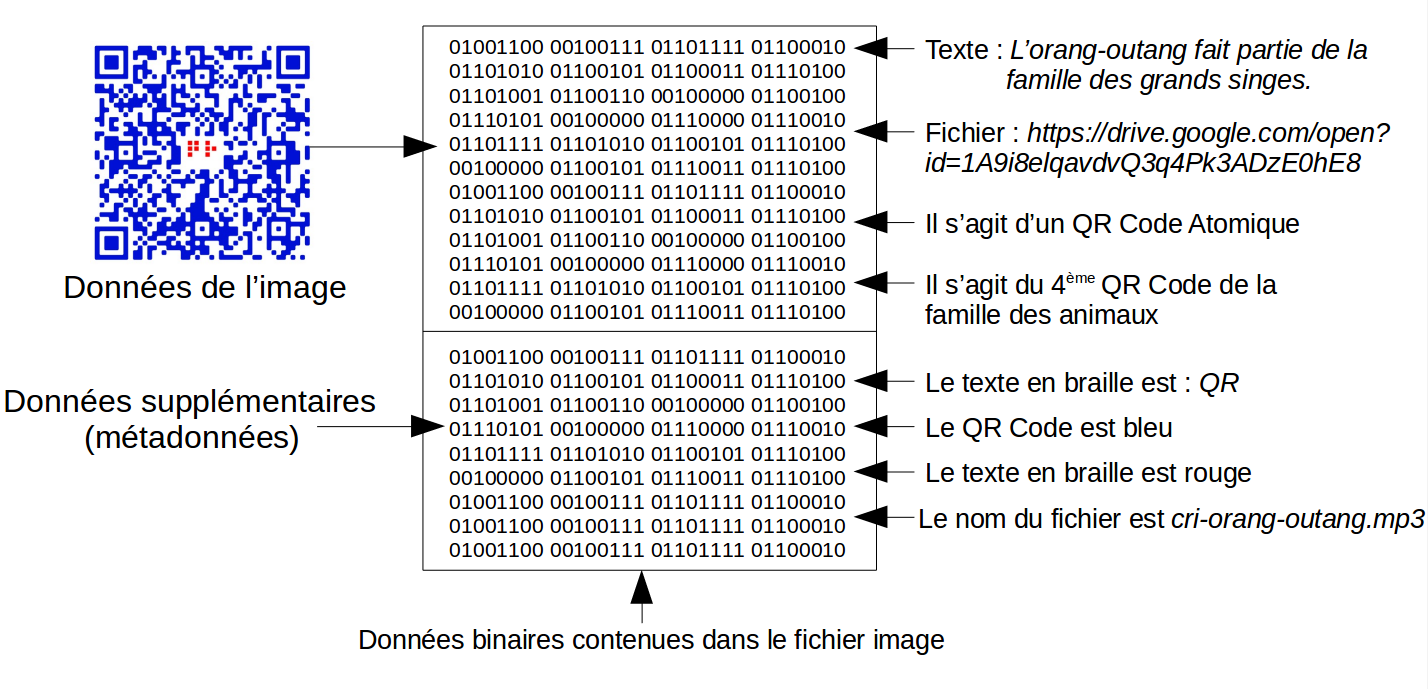
\includegraphics[scale=0.33]{img/schema_representation_donnees.png}
   \caption{Contenu d'une image d'un QR Code}
\end{figure}

\newpage
\par
Afin de stocker ces données de manière formelle, nous avons établi une structure de type XML\footnote{eXtensible Markup Language (https://www.w3schools.com)} (voir \ref{compression}). Elle fait apparaître clairement la dichotomie entre les données stockées dans le QR Code (noeud \noeud{donneesUtilisateur}) et les données stockées dans les métadonnées de l'image (noeud \noeud{metadonnees}).
\par
Le type de QR Code (atomique ou ensemble) est indiqué par un attribut dans le noeud \noeud{donneesUtilisateur}. Ce noeud contient un noeud \noeud{contenu} contenant lui-même un ensemble de textes (\noeud{texte}) et de fichiers (\noeud{fichier}).
\par
L'appartenance à une famille (voir \ref{typesQR}) de QR Codes est indiquée par la présence d'un noeud \noeud{famille} ayant pour attributs le nom de la famille et la place du QR Code.
\par
La représentation formelle de l'exemple du QR Code orang-outang est visible dans la figure ci-dessous.

\begin{figure}[!h]
\begin{adjustbox}{minipage=\textwidth,bgcolor={RGB}{240 240 240}}

\lstset{language=XML}

\begin{lstlisting}
<qrcode>
  <donneesutilisateur type="atomique">
    <contenu>
      <texte>L'organg-outang fait partie de la famille 
             des grands singes.</texte>
      <fichier url="1A9i8elqavdvQ3q4Pk3ADzE0hE8"/>
    </contenu>
    <famille nom="animaux" ordre="4"/>
  </donneesutilisateur>
  <metadonnees>
    <fichiers>
      <fichier url="1A9i8elqavdvQ3q4Pk3ADzE0hE8" 
               nom="cri-orang-outang.mp3"/>
    </fichiers>
    <colorqrcode color="#1606e7"/>
    <textebraille texte="QR"/>
    <colorbraille color="#ea0000"/>
  </metadonnees>
</qrcode>
\end{lstlisting}

\end{adjustbox}
\caption{Représentation d'un QR Code}

\end{figure}\textbf{}